
\documentclass{discussion}

%% MODIFY:  Document-specific Packages ----------------------------------------------

% References
% \usepackage{biblatex}
\usepackage{natbib}
% \addbibresource{dis02_references.bib}

%% MODIFY:  Document-specific Commands ----------------------------------------------
\renewcommand{\a}{\mathbf{a}}
\renewcommand{\u}{\mathbf{u}}
\renewcommand{\b}{\mathbf{b}}
\newcommand{\z}{\mathbf{z}}

%%%%%%%%%%%%%%%%%%%%%%%%%%%%%%%%%%%%%%%%%%%%%%%%%%%%%%%%%%%%%%%%%%%%%%%%%%%%%%%%%%%%%
\begin{document}

%% MODIFY: Lecture Info -------------------------------------------------------------
\lecture{2}{Probability \& Bayesian Paradigm}{Benjamin Bray and Chansoo Lee}

%%%% TWO APPROACHES %%%%%%%%%%%%%%%%%%%%%%%%%%%%%%%%%%%%%%%%%%%%%%%%%%%%%%%%%%%%%%%%%
\section{Writing Mathematical Proofs}

Online Resources:
\begin{itemize}
\item Prof. John Lee at University of Washington has an excellent writeup focusing on writing techniques. \href{https://www.math.washington.edu/~lee/Writing/writing-proofs.pdf}{[link]}
\item Prof. Michael Hutchings at UC Berkeley has a more beginner-friendly writeup which includes basic proof templates. \href{https://math.berkeley.edu/~hutching/teach/proofs.pdf}{[link]}
\end{itemize}

Important things
\begin{itemize}
\item Do NOT start by stating the conclusion of an implication you are trying to prove. When you  prove $p$ implies $q$, $q$ should NEVER appear until the very end of the proof.
\item Define variables (e.g. let $a$ be a real number) when they appear first time. In C/JAVA, you'd get a compile time error which prevents you from even \emph{submitting} a proof with undefined variables. In math proofs, you will get instead a \emph{run-time} error when readers try to understand your proof, like in Python. Remember that variables have no meaning until you define them.
\item Explain your logic with English sentences instead of ambiguous math symbols such as $\therefore$ and $\because$.  You wouldn't want your collaborators to write even more code when they \emph{document} their code.
\end{itemize}

\section{Probability Notations}
We will review the essential probability definitions using two-dice example.

\newcommand{\var}{\mathrm{Var}}
\renewcommand{\E}{\mathbb{E}}

\begin{itemize}
\item \textbf{Random variable} is denoted by capital letters such as $X$ and $Y$.
\item \textit{Sample space} $\Omega(X)$ is the \textit{set} of values that $X$ can take.
\item An \textbf{Event} is a subset of sample space. Events are also denoted by capital letters such as $A$ or $B$. We often omit the set notations. For example, $(X = x)$ is the event $\{x\}$, and $(a \leq X \leq b)$ is the event $\{x \in \Omega(X): a \leq x \leq b\}$.
\item \textbf{Probability of an event} is denoted by $P(A)$.
\item \textbf{Joint probability}, denoted by $P(A,B)$, is the probability that the event $A$ and $B$ both happen.
\item \textbf{Conditional probability} of an event, $P(A | B) = P(A \cap B) / P(B)$ is the probability that $A$ happens given $B$ happens.
\item Two events are \textbf{independent} if $P(A | B) = P(A)$. \textit{Question:} What does it imply about $P(A \cap B)$?
\item \textbf{Probability mass function (pmf)} of a discrete random variable, denoted by $f_X$, $\mu_X$, or $p_X$, maps each element $x \in \Omega(X)$ to the probability that $X = x$.
\item \textbf{Joint probability mass function} of two discrete random variables, denoted by $f_{X,Y}(x, y)$, maps each element in $(x,y) \in \Omega(X) \times \Omega(Y)$ to the probability that $(X,Y) = (x,y)$.
\item \textbf{Conditional mass function} is defined as $f_{X|Y}(x | y) = f_{X,Y}(x,y) / f_Y(y)$.
\item \textbf{Expectation} of $X$ is defined as:
\[\E[X] = \sum_{x \in \Omega(X)} f_X(x) x \]
\item \textbf{Conditional expectation} of $X$ given $Y$ is a function of $Y$ defined as:
\[\E[X | Y] = \sum_{x \in \Omega(X)} f_{X | Y}(x) x \]
\item \textbf{Variance} of $X$ is defined as: $\var[X] = \E[(X - \E(X))^2].$
\end{itemize}

\vspace{1em}

\begin{exercise}
Throw two dice and define $X_1$ and $X_2$ to be the result of each. Let $M = \max(X_1, X_2)$ and $S = X_1 + X_2$. Find 
\begin{itemize}
\item $\E[X_2 | X_1]$
\item $\E[S | X_1]$
\item $\E[M | X_1]$
\item $\E[S | X_2$ is even]
\end{itemize}
\end{exercise}

\vspace{1em}


\begin{exercise}
Let $X,Y,Z$ be random variables and $a,b$ be real numbers. Show the linearly of conditional expectation: $\E[aY + bZ | X] = a\E[Y | X] + b\E[Z | X]$.
\end{exercise}

\vspace{1em}

\begin{exercise}
Show that $\var(X | Y) = E(X^2 | Y) - [E(X | Y)]^2$.
\end{exercise}

\subsection*{Remarks}
\begin{itemize}
\item We sometimes omit the subscripts for pmfs and deduce them from the context. For example, $f(x,y)$ is the joint density function.
\item For a continuous random variable, we have a \textbf{(conditional/joint) probability density function} instead. But we can't really explain it in this course. Generally speaking, however, things that hold for pmfs also hold for pdfs, after converting summations $\sum_{x \in \Omega(X)}$  to integrals $\int_{\Omega(X)} \ dx$.
\item One important difference is that the probability of event $X = x$ for any $x \in \Omega(X)$ is 0, so pdf does \textit{not} define the probability that $X = x$.
\end{itemize}


For more on discrete random variables, read \href{http://ocw.mit.edu/courses/mathematics/18-05-introduction-to-probability-and-statistics-spring-2014/readings/MIT18_05S14_Reading3.pdf}{this}. For more on continuous random variables, read \href{http://www.math.uah.edu/stat/expect/Conditional.html}{this}.

\section{Two Approaches to Data Analysis}

There are two cultures in the use of statistical modeling to reach conclusions from data \citep{breiman2001}, each differing in their goals and assumptions.  We are typically given a vector of input variables $\X$ and the corresponding response variables $\Y$, which have been created by nature in response to the input variables. Once we have a dataset, we may be interested in either the \textbf{prediction} of response variables for future input variables or in extracting \textbf{information} about how nature is associating the response variables with the input variables from within its black box.

\begin{figure}[h!]
    \centering
    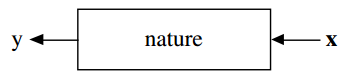
\includegraphics[width=150px]{images/nature-black-box}
    \caption{Data is generated by a black box that we cannot peek inside of.}
    \label{fig:nature-black-box}
\end{figure}

%% Data Modeling --------------------------------------------------------------------
\subsection*{Data Modeling Culture}

There are two different approaches toward these goals.  Analysis in the \textbf{data modeling culture} (i.e. most statisticians) makes assumptions about the data is generated from within nature's black box, often using a statistical model to do so.  For example, a common data model is that observed data is generated by independent draws from a known family of probability distributions, with some parameters $\theta$ that can be tuned to fit the data.
%
\begin{align*}
    \X &\quad \text{ input variables} \\
    \eps &\quad \text{ random noise} \\
    \theta &\quad \text{ parameters} \\
    \Y &\sim f(\X, \eps, \theta)
\end{align*}

Once the values of the parameters are estimated from the data, the model can be used for information or prediction.  Different data models work best in different settings, and care must be taken to choose an appropriate model.  Statisticians use \textit{goodness-of-fit} tests to check that their data models do not make wildly inappropriate assumptions about the data.  Many classical statistical models fall under this category, including linear regression, logistic regression, mixture models, and generative probabilistic graphical models in general.

%% Algorithmic Modeling -------------------------------------------------------------
\subsection*{Algorithmic Modeling Culture}

Analysis in the \textbf{algorithmic modeling culture} (i.e. most computer scientists) assumes that the inside of the black box is far too complex and unknown to model directly.  Instead, their approach is to find an algorithm $f(\X)$ that operates on the input variables to predict the response variables.  Because algorithmic modelers are willing to sacrifice interpretability of their models for higher accuracy, they are more able to take advantage of powerful, one-size-fits-most techniques like deep neural nets and random forest models.

\begin{figure*}[h!]
    \centering
    \begin{subfigure}[t]{0.5\textwidth}
        \centering
        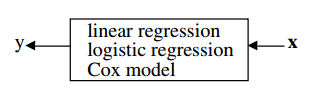
\includegraphics[width=150px]{images/data-model}
        \caption{Data modelers make assumptions about how the black box generates the response variables.  If the model does not reflect nature, this approach will perform poorly.}
    \end{subfigure}%
    ~ 
    \begin{subfigure}[t]{0.5\textwidth}
        \centering
        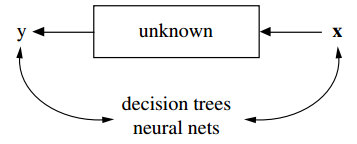
\includegraphics[width=150px]{images/algorithmic-model}
        \caption{Algorithmic modelers don't care whether or not their model reflects the data generating process, only that it performs well at prediction tasks.}
    \end{subfigure}
\end{figure*}

%% Which Approach is Better? --------------------------------------------------------
\subsection*{Which Approach is Better?}

Each approach to data analysis has its merits, and this is a vastly oversimplified view of how researchers and data scientists solve problems.  Data models give statisticians a peek into nature's black box, and allow for greater interpretability.  It is also much easier to provide confidence intervals for a data model, which can be important in domains like medicine.  Algorithmic models are more capable of modeling complicated data like images and speech, although it is harder to make guarantees about the results.  This semester, we will give you a chance to solve problems using both approaches, and you can weigh for yourself the relative advantages and disadvantages of each.

%%%% PROBABILISTIC MODELING %%%%%%%%%%%%%%%%%%%%%%%%%%%%%%%%%%%%%%%%%%%%%%%%%%%%%%%%%
\section{Probabilistic Modeling: Maximum Likelihood}

Let $\mathcal{D}$ be a family of distributions over $n$ samples, parametrized by $\theta$, where each element has joint pmf(pdf) $p(\cdot;\theta)$ over $n$ samples. \textbf{Likelihood} is a function of the distribution parameter $\theta$ given samples (data) $X_1, \ldots, X_n$:
\[L(\theta; X_1, \ldots, X_n) = p(X_i, \ldots, X_n; \theta).\]
We mostly consider a special case of \emph{product distributions}, where $\mu_\theta(X_i, \ldots, X_n) = \prod_{i=1}^{N} p(X_i;\theta).$

The maximum likelihood estimate $\hat{\theta}_{ML}$ is simply the maximizer for $L(\theta)$. It is the parameter value under which the observed data is most probable.

% We take the log-likelihood for many reasons; it converts multiplication to addition; avoids numerical underflow on a computer when multiplying lots of small probabilities together.  Maximizing log likelihood is equivalent to maximizing likelihood.

%% Maximum Likelihood ---------------------------------------------------------------


\textbf{Discuss:} Instead of the likelihood, we use the log likelihood $\L(\theta|\X) = \log P(\theta|\X)$. Can you explain why?

\vspace{1em}

\begin{exercise}(Discrete)
Suppose we observe the result of $N$ flips of a coin with unknown bias $\theta$ (probability of heads).
\begin{enumerate}
\item Write the likelihood function for this example.
\item Differentiate to find the MLE. 
% Show that $\hat{\theta}_{ML} = \frac{1}{N}\sum_{k=1}^N x_k$.  (easiest with log-likelihood rather than likelihood.  Use the trick $P(x_k | \theta) = \theta^{x_k} (1-\theta)^{1-x_k}$.
\end{enumerate}
\end{exercise}

\paragraph{Remark}When asked to estimate parameters, it always helps to write down the corresponding data model.  This involves identifying the relevant probability distributions and any other variables that may influence the result.  Here, we can use the \textbf{Bernoulli distribution} $\Ber[\theta]$ to model the result of a single coin flip.
    \begin{align*}
    \theta &\sim \text{fixed parameter} & \text{(bias of coin)} \\
    X_1, \dots, X_N &\iid \Ber[\theta] & \text{(coin flips)}
    \end{align*}


\vspace{.5em}

\begin{exercise}(Continuous and bounded)
Suppose we observe $N$ samples from uniform distribution over $[0, \theta]$. What is the MLE of $\theta$?  Hint: $L(\theta) = \theta^{-n}$.
\end{exercise}

\vspace{.5em}

\begin{exercise}(Continuous and unbounded)
Suppose we observe $N$ samples from the density function $p(x;\theta) = \frac{1}{2\theta} \exp(-|x| / \theta).$ What is the MLE of $\theta$?
\end{exercise}

\paragraph{Remark} Remember that $\theta$ can be any mathematical object, such as:
\begin{itemize}
\item scalar, as in all examples above.
\item vector, e.g. $(\mu,\sigma) \in \R^2$ when $\mathcal{D}$ is one-dimensional Gaussian.
\item vector and matrix, e.g. $(\mu, \Sigma) \in \R^m \times \R^{m \times m}$ for mean vector and covariance matrix when $\mathcal{D}$ is multidimensional Gaussian.
\end{itemize}
If $L$ is a function of more than one variable, then the MLE requires optimizing over all variables.

% %% Maximum a Posteriori -------------------------------------------------------------
% \subsection*{Maximum a Posteriori Estimation}

% %% Example:  Motivation for Priors
% \begin{example}
% Suppose we observe the result of $N=1$ coin flip.  What problems might the maximum likelihood approach have in this setting?
% \end{example}

% \begin{answer}
% If the flip comes up heads, then $\hat\theta_{ML} = 1$.  If we observe tails, then $\hat\theta_{ML} = 0$.  We have a \textit{data sparsity} problem--there is not enough data to make an informed decision about the problem.  Given our prior knowledge of coins, these estimates are unlikely to be correct unless both sides of the coin are identical.
% \end{answer}

% \begin{enumerate} \color{red}
% \item Explain what a Bayesian prior is and how to interpret it.  
% \item A prior explicitly summarizes our assumptions about the problem before we see any data.  The MAP estimate will be an interpolation between our prior and the maximum likelihood estimate.  We can use a strong prior or a weak prior.  The stronger our prior, the more data we must observe to overcome our prior assumptions.  (Example:  A grandma has seen many coin flips and will need many observations to convince herself that the coin presented to her is biased.  A baby has not seen many coins before, and will believe that a coin is biased after only a few flips.)
% \item Review the Beta distribution.  Domain, range, mean, mode.  Interpretation as a prior.  Conjugacy with the Binomial distribution.
% \end{enumerate}

% %% Example:  Bayesian Priors
% \begin{example}
% Suppose we observe the result of $N$ flips of a coin with unknown bias $\theta$ (probability of heads). 
% Assuming a $\Beta(a,b)$ prior on $\theta$, what is the MAP estimate of $\theta$?
% \end{example}

% \begin{enumerate} \color{red}
% \item $\hat{\theta}_{MAP} = \frac{a + \sum x_k}{a+b+N}$.  (there may be some -1 factors in there that I'm missing.)
% \item Interpretation of MAP estimate for binomial/bernoulli:  The prior explicitly encodes the assumption that we've seen $a+b$ coin flips in our life, $a$ of which turned up heads.  That's why the parameters are sometimes called \textbf{pseudocounts}.
% \end{enumerate}

%% Bayesian Inference --------------------------------------------------------------- 
% \subsection*{Bayesian Inference}

% \begin{enumerate} \color{red}
% \item There probably isn't enough time for this, but maybe mention posterior distributions etc.  Refer to Murphy MLAPP Ch 3 or Ch 5.
% \end{enumerate}


%%%% REFERENCES %%%%%%%%%%%%%%%%%%%%%%%%%%%%%%%%%%%%%%%%%%%%%%%%%%%%%%%%%%%%%%%%%%%%%

% Bibliography
\bibliographystyle{plainnat}
\bibliography{dis02_references}
\end{document}
